\section{Generalized Autoregressive Conditional Heteroskedasticity Model}
\label{sec:GARCH}
The Generalized Autoregressive Conditional Heteroskedasticity (GARCH) model is structured as an ARMA model applied to the variance of the error term, relying on the previous squared error terms and variances. \\
Formally, the GARCH model of order $(p, q)$ is defined as:
\begin{equation}
    \label{eq:GARCH}
    \sigma^2_t = a_{0} + \sum^{p}_{i=1} a_i \epsilon^2_{t-i} + \sum^{q}_{j=1} a_{j+p} \sigma^2_{t-j}
\end{equation}
Here, $p$ is the number of past squared error terms considered, $q$ is the number of past variances considered, $a_0, a_1, ..., a_{p+q}$ are the model parameters, $\epsilon^2_{t-1}, \epsilon^2_{t-2}, ..., \epsilon^2_{t-p}$ are the past squared error terms, and $\sigma^2_{t-1}, \sigma^2_{t-2}, ..., \sigma^2_{t-q}$ are the past variances. \\
For our analysis, we assumed that the error terms $\epsilon_t$ are independent and identically distributed variables from a normal distribution with mean $0$ and variance $\sigma^2_t$, i.e., $\epsilon_t \stackrel{iid}{\sim} \mathcal{N}(0,\sigma^2_t)$.
\subsection*{AR(1) + GARCH(1,1)}
We applied the GARCH(1,1) model to the variance of the error term in an AR(1) model, leading to the following likelihood:
\begin{equation}
    \label{eq:GARCH1,1_likelihood}
    y_{t}|\mu_{0},\alpha,y_{t-1},a_0,a_1,a_2,\sigma^2_{t-1} \sim \mathcal{N}(\mu_{0} + \alpha y_{t-1}, a_0 + a_1 \epsilon^2_{t-1} + a_2 \sigma^2_{t-1})
\end{equation}
For the priors, we chose:
\begin{equation}
    \label{eq:GARCH1,1_priors}
    \begin{split}
        \mu_0 \sim \mathcal{N}(0.0, 10000) \\
        \alpha \sim \mathcal{U}(-1.0, 1.0) \\
        a_0 \sim \mathcal{G}(0.01, 0.01) \\
        a_1 \sim \mathcal{G}(0.01, 0.01) \\
        a_2 \sim \mathcal{G}(0.01, 0.01)
    \end{split}
\end{equation}
The gamma distribution is used for $a_0, a_1, a_2$ to ensure positive variance values. The normal and uniform distributions for $\mu_{0}$ and $\alpha$, respectively, are chosen for the same reasons as in the AR(1) model discussed in Section \ref{sec:AR}. \\
Running the JAGS code to implement the AR(1) + GARCH(1,1) model for GDP and CPIAUCSL, we obtained the posterior distributions shown in Figure \ref{fig:GARCH1,1_AR1_posteriors}, with the corresponding means and 95\% credible intervals reported in Table \ref{tab:GARCH1,1_AR1_posteriors}. Trace plots are provided in the Appendix. \\
\begin{figure}[H]
    \centering
    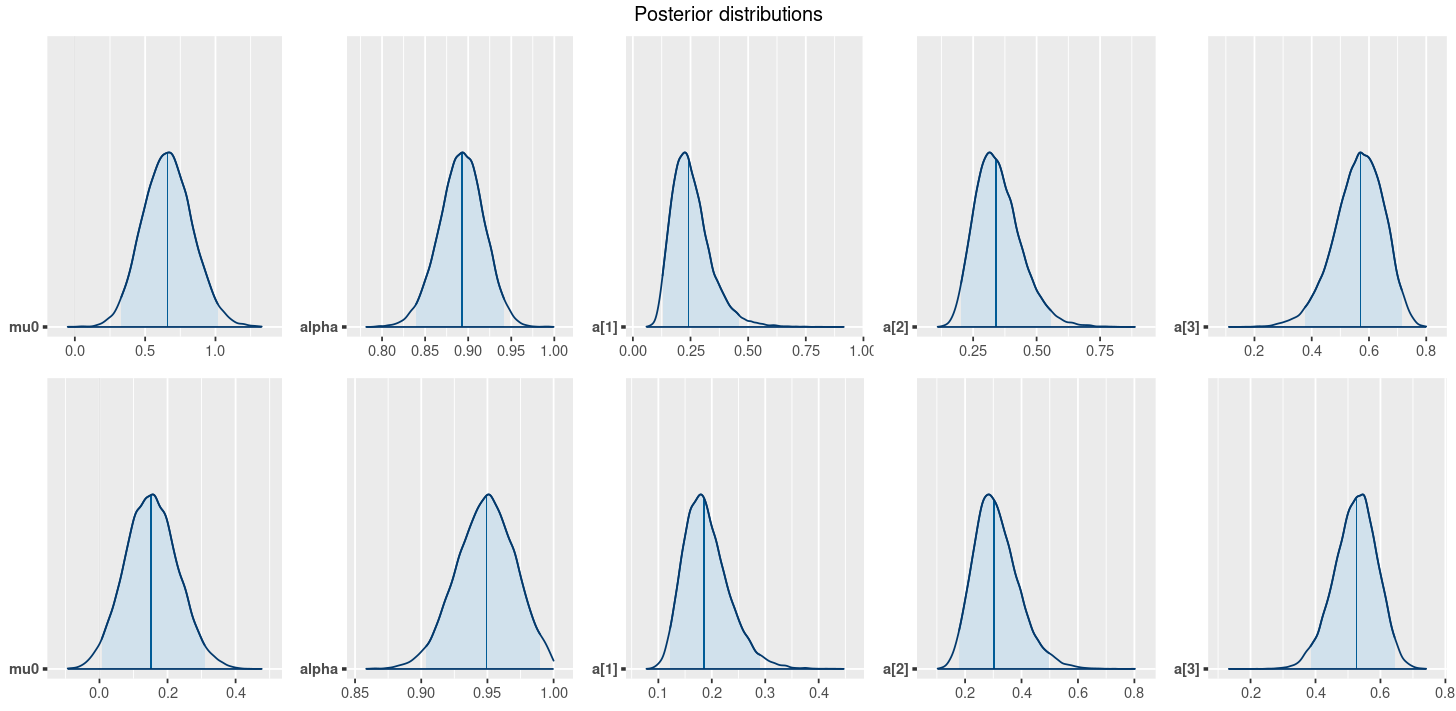
\includegraphics[width=\textwidth]{images/5-GARCH/posteriors.png}
    \caption{Posterior distributions of the parameters for the AR(1) + GARCH(1,1) models. The top line corresponds to the model used for GDP, while the bottom line corresponds to the model used for CPIAUCSL.}
    \label{fig:GARCH1,1_AR1_posteriors}
\end{figure}
\begin{table}[H]
    \centering
    \begin{tabular}{c|c|c|c}
        \textbf{Model target variable } & \textbf{Parameter } & \textbf{Posterior Mean } & \textbf{95\% Credible Interval } \\
        \cline{1-4}
        GDP      & $\mu_0$  & 0.6607917 & (0.330124347, 1.0149443) \\
        GDP      & $\alpha$ & 0.8922917 & (0.839581644, 0.9416944) \\
        GDP      & $a_1$    & 0.2543789 & (0.128699457, 0.4589058) \\
        GDP      & $a_2$    & 0.3492357 & (0.202666918, 0.5555133) \\
        GDP      & $a_3$    & 0.5641981 & (0.377027833, 0.7144185) \\
        CPIAUCSL & $\mu_0$  & 0.1533340 & (0.006694284, 0.3087467) \\
        CPIAUCSL & $\alpha$ & 0.9485379 & (0.903837995, 0.9896255) \\
        CPIAUCSL & $a_1$    & 0.1904433 & (0.122120513, 0.2894240) \\
        CPIAUCSL & $a_2$    & 0.3120365 & (0.179010077, 0.4966238) \\
        CPIAUCSL & $a_3$    & 0.5232054 & (0.384775889, 0.6435153) \\
    \end{tabular}
    \caption{Posterior means and 95\% credible intervals for the parameters of the AR(1) + GARCH(1,1) models.}
    \label{tab:GARCH1,1_AR1_posteriors}
\end{table}
Plotting the in-sample and out-of-sample predictions with 95\% credible intervals and comparing them with the actual data, we obtained the results shown in Figures \ref{fig:GARCH1,1_AR1_gdp_prediction} and \ref{fig:GARCH1,1_AR1_infl_prediction}. The results from the AR(1) + GARCH(1,1) model are not significantly different from those obtained using the AR(1) model, suggesting that the AR(1) model already captures most of the information present in the data. \\
\begin{figure}[H]
    \centering
    \begin{minipage}{0.49\textwidth}
        \centering
        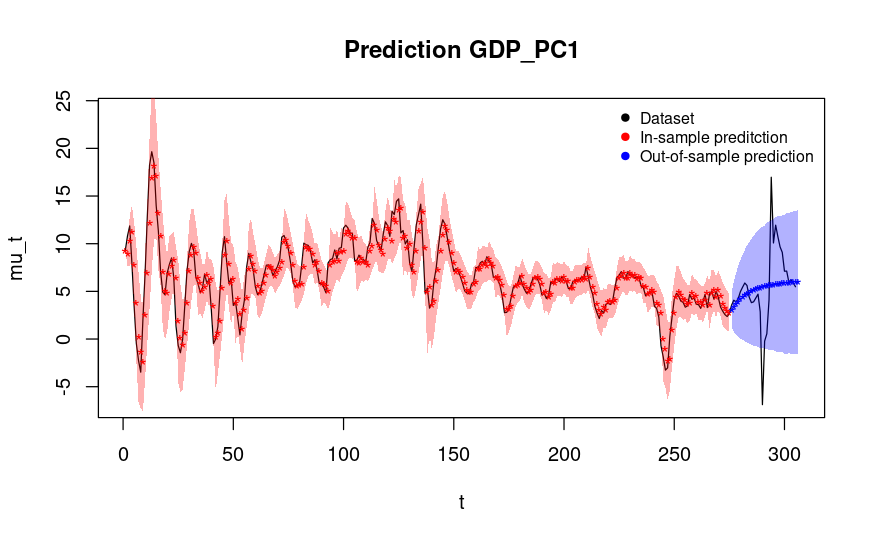
\includegraphics[width=\textwidth]{images/5-GARCH/gdp_prediction.png}
        \caption{In-sample and out-of-sample predictions for the GDP using the GARCH(1,1) + AR(1) model.}
        \label{fig:GARCH1,1_AR1_gdp_prediction} 
    \end{minipage}\hfill
    \begin{minipage}{0.49\textwidth}
        \centering
        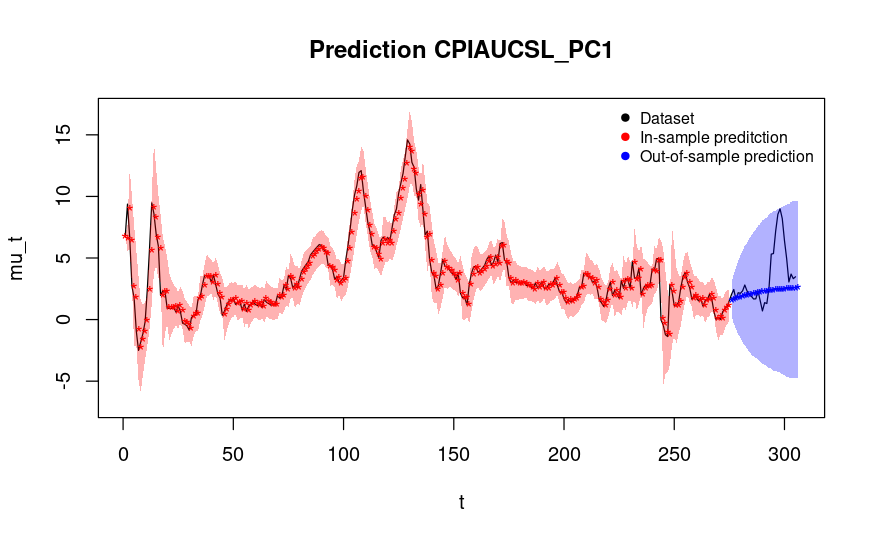
\includegraphics[width=\textwidth]{images/5-GARCH/infl_prediction.png}
        \caption{In-sample and out-of-sample predictions for the CPIAUCSL using the GARCH(1,1) + AR(1) model.}
        \label{fig:GARCH1,1_AR1_infl_prediction}
    \end{minipage}
\end{figure}
Lastly, we compared our model with the results obtained from the uGarch library and found no significant differences in the in-sample predictions of both approaches. However, the analysis did reveal slight differences in the parameter estimates.